\section{Устройство системы}
\label{sec:Chapter4} \index{Chapter4}

\subsection{Дерево структурной разметки документа}

Каждая вершина дерева структурной разметки имеет следующие поля: тип, текст содержимого и список вершин - сыновей и вершину-родителя. Изначально текст содержимого для вершины не определен, и заполняется в том случае, если в процессе переноса фрагментов требований вызывалась функция получения текста раздела, описанная ниже. Тип вершины дерева не фиксирован и зависит от соответствующей вершины DOM модели. Тремя зафиксированными типами вершин являются: 

\begin{itemize}

\item \textbf{"text"} - в случае если вершина содержит текстовую информацию. Может находиться только в листьях дерева. Если тип вершины - \emph{"text"}, в ней заполняется специальное поле, в котором запоминается содержимое соответствующего вершине участка текста документа.

\item \textbf{"body"} - содержится в единственном экземпляре в корне дерева.

\item \textbf{"requirement"} - в случае, если вершина содержит фрагмент требования. Может иметь только одного потомка типа \emph{"text"}. Если тип вершины - \emph{"requirement"}, в ней заполняются специальные поля, служащие для формирования списка требований и дальнейшего переноса фрагмента во в конечный документ.

Поле id содержит идентификационный номер требования, к которому относится фрагмент, соответствующий вершине. Поле a содержит \emph{true} или \emph{false} в зависимости от того, нужно ли добавлять пару тегов ссылки на требование \newline(\emph{<a name="***" id="***" class=”requality\_id”></a>}) после переноса фрагмента в конечный документ. 

\end{itemize}

\subsection{Построение дерева структурной разметки по DOM модели документа}

Построение вершин дерева структурной разметки осуществляется в порядке обхода DOM дерева в глубину \cite{book:Programming}. При этом вершины, не влияющие на структуру документа, игнорируются и не участвуют в построении дерева структурной разметки. В данной работе к вершинам, влияющим на структуру документа, вершины DOM модели документа, имеющие имена \emph{"span"\, "a" (в случае, когда вершина с именем "a" является потомком вершины, соответствующей фрагменту требования)\, "h1---h6"\, "p"\, и "blockquote"}. Соответствующая вершина дерева структурной разметки создается на основе текущей рассматриваемой вершины DOM модели.

Для организации иерархии параграфов и разделов используется стек (эта структура данных подробно описана в \cite{book:Programming}): При прохождении в DOM дереве вершины заголовка раздела проверяется, есть ли такой тип раздела в стеке. Если его нет, то считается, что текущий раздел является подразделом последнего встреченного раздела и соответствующая ему вершина добавляется в стек. В противном случае из стека извлекаются вершины дерева до тех пор, пока извлеченная вершина не будет иметь тот же тип, что и добавляемая, а затем родителем добавляемой вершины становится родитель извлеченной из стека. Таким образом вершины подразделов одного и того же раздела в дереве структурной разметки имеют одинаковую глубину.

В случае, если текущая рассматриваемая вершина DOM модели документа имеет имя \emph{span} и атрибут \emph{class}, начинающийся с \emph{"requality\_text"}, в дереве разметки создается вершина, имеющая тип requirement, и в ней заполняются поля \emph{id} и \emph{a}. По умолчанию считается, что такие вершины содержатся только в исходном документе.

\subsection{Устройство требования}

\begin{itemize}
\item \textbf{Фрагмент требования (Location)}

Объект этого типа содержит ссылку на соответствующую фрагменту вершину дерева разметки. Предоставляет метод, позволяющий определять порядковый номер вершины в списке сыновей её родителя.

\item \textbf{Объединение фрагментов (ActualLocation)}

В силу особенностей выделения фрагментов требований в системе Requality, подряд идущие участки текста, соответствующие одному требованию, могут находиться в разных фрагментах из-за наличия разметки. Перед переносом такие участки нужно объединить в один, для которого и должен осуществляться поиск соответствия в конечном документе.

\item \textbf{Требование (Requirement)}

Объект каждого требования содержит \emph{id} требования, список фрагментов, относящихся к нему, и список объединений фрагментов, полученный в результате обработки списка фрагментов. Объединение фрагментов происходит в том случае, если они имеют общего родителя, и их порядковые номера, как сыновей, отличаются на единицу. Помимо этого, объект типа Requirement содержит информацию о том, нужно ли добавлять пару тегов ссылки на требование, при переносе этого фрагмента.  

\end{itemize}

\subsection{Извлечение текста из дерева структурной разметки}

Текстом вершины X дерева структурной разметки будем называть объединение полей text тех вершин дерева, которые имеют тип text и содержатся в поддереве, корнем которого является вершина X.

\begin{enumerate}
\item \textbf{Текст заголовка}

Текстом заголовка считается объединение текстов всех подряд идущих вершин, являющихся прямыми потомками вершины, соответствующей этому заголовку, до первой вершины, соответствующей абзацу. На рисунке \ref{sys:headertext} фрагмента дерева разметки выделены вершины, текст которых участвует в тексте заголовка h1.

\begin{figure}[h]
\begin{center}
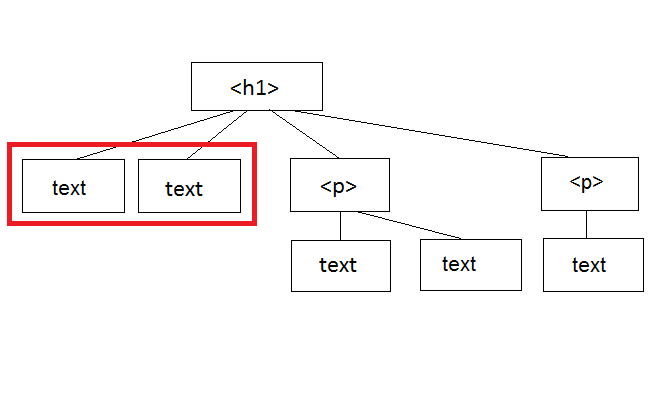
\includegraphics[scale=0.7]{headerText.png}
\caption{Текст заголовка дерева разметки}
\label{sys:headertext}
\end{center}
\end{figure}

\item \textbf{Текст раздела}

Текст раздела содержит в себе текст соответствующего заголовка и текст всех вершин, не являющихся подзаголовками этого раздела. На рисунке \ref{sys:parttext} фрагмента дерева разметки выделены вершины, текст которых включается в текст раздела h1.

\begin{figure}[h]
\begin{center}
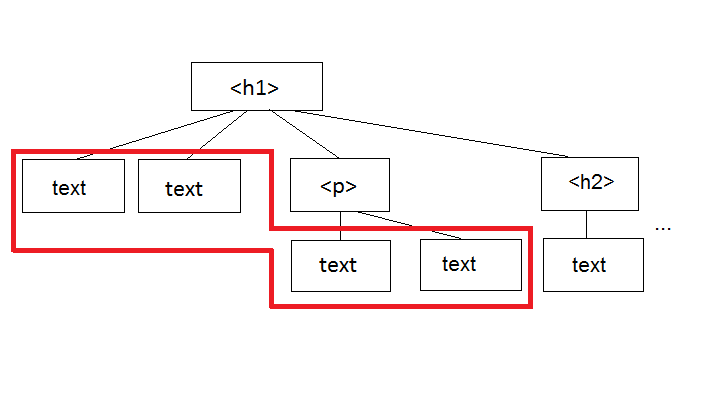
\includegraphics[scale=0.7]{partText.png}
\caption{Текст раздела дерева разметки}
\label{sys:parttext}
\end{center}
\end{figure}

После получения текста раздела он преобразуется при помощи регулярных выражений и запоминается в специальном поле соответствующей вершины дерева структурной разметки документа.

\item \textbf{Использование регулярных выражений}

Поскольку используемые незначащие символы в исходном и конечном документах могут отличаться, для осуществления сравнения и поиска в частях текстов их необходимо привести к унифицированному виду. Для этого используется механизм регулярных выражений, описанный в \cite{book:RegExp}, \cite{web:Reg}. Перед дальнейшим использованием текста раздела или заголовка, над ним осуществляются следующие преобразования:

\begin{itemize}
\item Все пробельные символы заменяются на пробел (символ ' ' в Java)

\item Удаляются все пробельные символы и переводы строк(whitespace characters) в начале и конце обрабатываемой строки

\item Несколько пробельных символов или переводов строк, идущих подряд, заменяются на один.

\item Пробельные символы, идущие перед знаками препинания, удаляются. После знаков препинания добавляется один пробел, если его нет.

\item Перед открывающими скобками добавляется один пробел, если его нет.

\item После открывающих и перед закрывающими скобками удаляется пробел, если он есть.
\end{itemize}

\end{enumerate}

\subsection{Устройство поиска соответствия объединению фрагментов требований}

По объединению фрагментов требования осуществляется поиск пути в дереве разметки исходного документа до подраздела, содержащего это объединение фрагментов. При этом из множества найденных путей выбирается тот, который имеет максимально возможную длину. Путь хранится в виде последовательности указателей на вершины дерева, начиная от корня. 

В дереве разметки конечного документа осуществляется поиск соответствующего пути. Путь B считается соответствующим пути A, если тексты всех заголовков в пути B совпадают с точностью до незначащих символов и цифр с текстами соответствующих заголовков в пути A. В случае если такой путь был найден, считается, что соответствие объединению фрагментов должно находиться в конечном документе в тексте подраздела, соответствующего последней вершине (вершине наибольшей глубины) найденного пути. В противном случае каждый фрагмент из этого объединения считается не перенесенным, и процесс переноса для данного объединения фрагментов требования останавливается.

Если в конечном документе путь, соответствующий пути до объединения фрагментов требования в исходном документе, был найден, то текст соответствующего подраздела конечного документа извлекается, преобразуется с использованием регулярных выражений, и в нём осуществляется поиск текста объединения фрагментов методом прямого поиска \cite{web:StrSearch}. Результатом поиска является позиция (номер символа), где в обработанном тексте подраздела начинается участок текста, полностью совпадающий с текстом объединения фрагментов требования, либо -1, если такая позиция не была найдена. По этой позиции далее осуществляется добавление тегов требований в конечный документ и элементов в соответствующее ему дерево разметки.

\subsection{Добавление элементов требований в дерево разметки документа}

В общем случае найденное соответствие объединению фрагментов лежит в нескольких вершинах дерева разметки конечного документа типа \emph{"text"}. Это объясняется тем, что вершины типа \emph{"text"}, идущие подряд, не объединяются при построении дерева разметки документа, при этом элементы DOM модели документа, не отвечающие за разметку, в построении дерева не используется. В ходе обхода поддерева, соответствующего найденному подразделу, возможны следующие варианты взаимного расположения найденного соответствия объединению фрагментов и вершин типа \emph{"text"}, и соответствующие проводимые операции:

\begin{enumerate}

\item Текст вершины дерева разметки не пересекается с найденным соответствием (находится до номера символа, с которого соответствие объединению фрагментов было найдено). В этом случае текст текущей рассматриваемой вершины пропускается.

\item Текст вершины дерева разметки полностью содержит в себе текст, соответствующий объединению фрагментов.

В этом случае осуществляется разбиение рассматриваемой текстовой вершины на три части (в общем случае, в частных случаях одна или обе пограничных текстовых вершины могут отсутствовать), согласно рисунку \ref{sys:add}, добавляется вершина требования (тип “requirement”) с соответствующим \emph{id}. Процесс преобразования дерева разметки для данного объединения фрагментов после проведения этой операции считается завершенным.

\begin{figure}[h]
\begin{center}
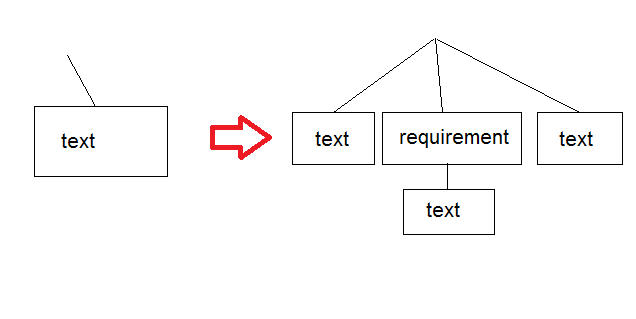
\includegraphics[scale=0.7]{add.png}
\caption{Случай полного вхождения текста объединения фрагметов в текстовую вершину дерева разметки}
\label{sys:add}
\end{center}
\end{figure}

\item Текст вершины дерева разметки частично содержит в себе текст, соответствующий объединению фрагментов. 

В этом случае осуществляется разбиение рассматриваемой текстовой вершины на две части (в общем случае, в частном случае одна пограничная текстовая вершина может отсутствовать) согласно рисунку \ref{sys:addNew}, добавляется вершина требования с соответствующим id. Затем часть текста, для которой была создана вершина типа requirement, удаляется из текста, соответствующего объединению фрагментов требования, и процесс продолжается для последующих текстовых вершин.

\begin{figure}[h]
\begin{center}
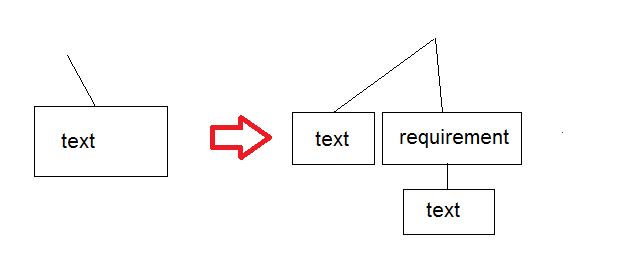
\includegraphics[scale=0.7]{addNew.png}
\caption{Случай неполного вхождения текста объединения фрагметов в текстовую вершину дерева разметки}
\label{sys:addNew}
\end{center}
\end{figure}

\end{enumerate}

\subsection{Добавление разметки требований в DOM модель}

По измененному дереву разметки конечного документа и его DOM дереву синхронно осуществляется обход в глубину - на каждом шаге обхода текущая рассматриваемая вершина дерева разметки соответствует вершине DOM дерева. В случае если рассматриваемая вершина дерева разметки и соответствующая ей вершина DOM дерева имеют тип \emph{"text"}, осуществляется проверка на совпадение содержимого текущих вершин DOM модели и дерева разметки. Если они не совпадают, считается, что эта вершина была изменена в дереве разметки конечного документа из-за добавления элементов требований, и вершину DOM дерева нужно разбить \cite{book:JDOM} на несколько таким же образом, как было описано в предыдущем пункте. Вершина типа \emph{"requirement"} дерева разметки при этом заменяется на вершину DOM дерева с именем \emph{span} и атрибутами \emph{class}, начинающимся \emph{"requality\_text"},  

Поскольку на данном этапе вершины дерева разметки и DOM дерева, тип которых отличен от \emph{"text"}, не влияют на работу этой части программы, их рассмотрение можно опустить, реализовав функции, получающие следующие в порядке обхода дерева в глубину вершины типа \emph{"text"} по текущим в дереве разметки и DOM дереве соответственно. 

После изменения DOM модели конечного документа по ней создается его измененная версия, содержащая теги перенесенных требований. 